\chapter{Árboles generadores de coste mínimo}
En este capítulo vamos a conocer algunos algoritmos (TAD partición, Kruskal o Prim) para obtener \textbf{grafos conexos acíclico}, es decir un árbol.

Es decir, dado un grafo no dirigido y conexo \(G = (V,A)\), se define un \textbf{árbol generador de G} (o de expansión) como un árbol que conecta todos los vértices de \(G\) sin que haya ciclos.

Su coste es la suma de los costes de las aristas del grafo.
\begin{figure}[h]
  \begin{center}
    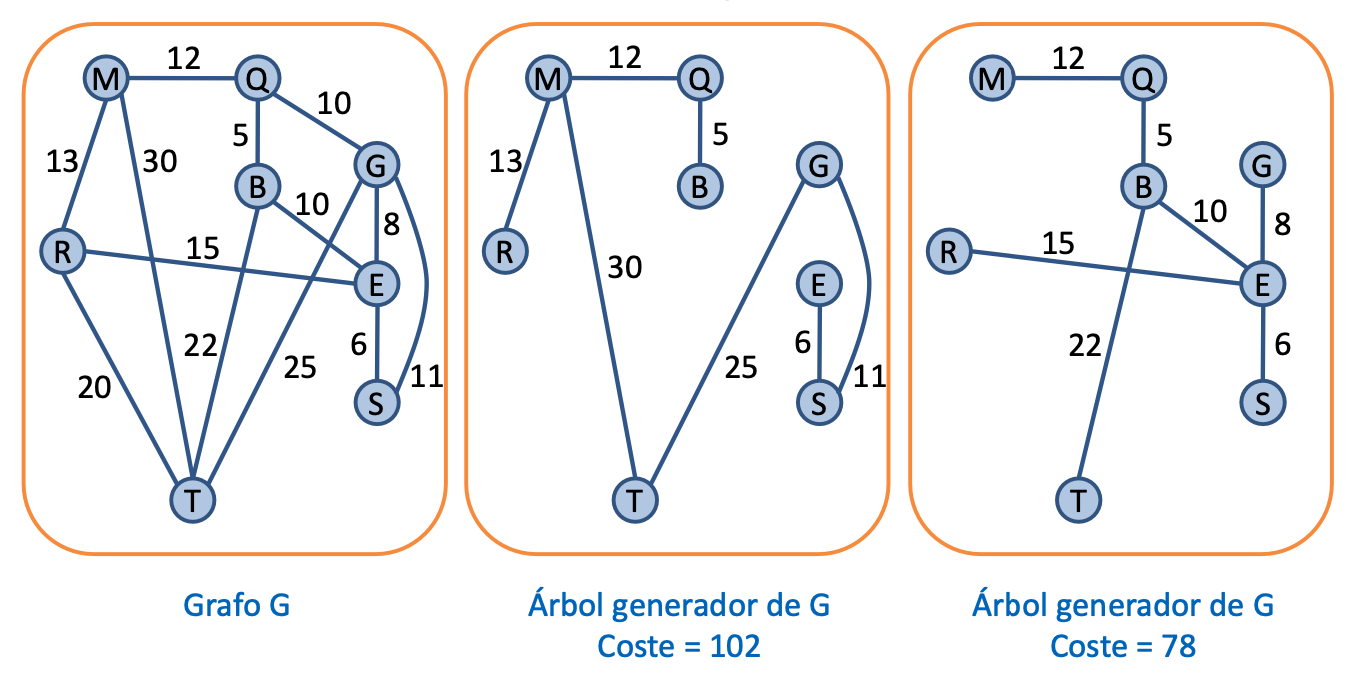
\includegraphics[width=.7\textwidth]{assets/AGCM.png}
  \end{center}
  \caption{Ejemplos de árboles generadores de coste mínimo}
\end{figure}

\section{TAD Partición}
Una \textbf{partición} es de un conjunto de enteros \(C = \{0,1,...,n-1\}\) es un conjunto de subconjuntos disjuntos, cuya unión es el conjunto total \(C\).

Encontramos la \textbf{enumeración de elementos} \(\rightarrow\) Definimos una aplicación \textit{biyectiva} (1a1) de un conjunto \(C\) en un rango de enteros \([0,n-1]\), tal que \(n\) es el cardinal de \(C\), mediante dos funciones:

\begin{figure}[h]
  \begin{minipage}{.4\textwidth}
    \begin{center}
      \verb|int IndiceElto(tElemento x);|
    \end{center}
    \underbar{\textit{Precondición:}} x \(\in\ C\).\\
    \underbar{\textit{Postcondición:}} Devuelve el índice del elemento x, en el rango \([0,n-1]\).
  \end{minipage}
  \hfill
  \begin{minipage}{.4\textwidth}
    \begin{center}
      \verb|tElemento NombreElto(int i);|
    \end{center}
    \underbar{\textit{Precondición:}} \(0 \leq i \leq n-1\).\\
    \underbar{\textit{Postcondición:}} Devuelve el elemento de \(C\) cuyo índice es i.
  \end{minipage}
\end{figure}
\newpage
\subsection{Especificación del TAD Partición}
Operaciones del TAD partición:

\textbf{Constructor de la partición}

\underbar{\textit{Postcondición:}} Crea una partición de subconjuntos unitarios en el intervalo de enteros \(0, n-1\).
\begin{center}
  \verb|Partición (int n);|
\end{center}

\textbf{Unir subconjuntos}

\underbar{\textit{Precondición:}} \(0 \leq a\), \(b \leq n-1\), a y b son los representantes de sus clases y \(a \neq b\).\\
\underbar{\textit{Postcondición:}}Une el subconjunto del elemento a y b en uno de los dos subconjuntos. La partición queda con un miembro menos.
\begin{center}
  \verb|void unir(int a, int b);|
\end{center}

\textbf{Buscar el representante de una partición}

\underbar{\textit{Precondición:}} \(0 \leq x \leq n-1\).\\
\underbar{\textit{Postcondición:}}Devuelve el representante del subconjunto al que pertenece \(x\).
\begin{center}
  \verb|int encontrar(int x) const;|
\end{center}


\subsection{Implementación del TAD Partición}
El TAD partición podemos implementarlo de diversas maneras (vector, listas, árboles,..), por tanto, vamos a ver como se implementan los algoritmos anteriores.

\textbf{Implementación mediante vector de pertenencia}

En cada posición del vector vamos a encontrar el representante de cada subconjunto.
\begin{figure}[h]
  \begin{center}
    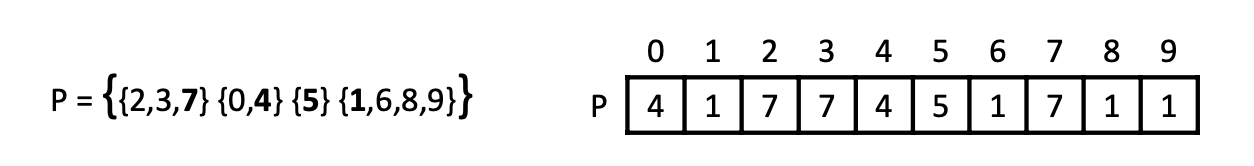
\includegraphics[width=\textwidth]{assets/impPAR1.png}
  \end{center}
  \caption{Ejemplo implementación vector de pertenencia}
\end{figure}

Vemos que en el subconjunto \(\{0,4\}\), en la posición `\textbf{0}' del vector, econtramos el representante `\textbf{4}', es decir, cada elemento en negrita es el representante del subconjunto.

Si queremos unir dos subconjuntos, primero llamaremos al método \texttt{encontrar()} y luego al método \texttt{unir()}.

El coste de las operaciones son:
\begin{itemize}
  \item \texttt{encontrar()} \(\in O(1)\), porque accedemos a la posición directamente.
  \item \texttt{unir()} \(\in O(n)\), porque recorremos todo el vector.
  \item \texttt{Partición()} \(\in O(n)\).
\end{itemize}
\newpage
Vamos a ver un ejemplo, uniendo los subconjunto de los elemento 4 y 1:
\begin{figure}[h]
  \begin{center}
    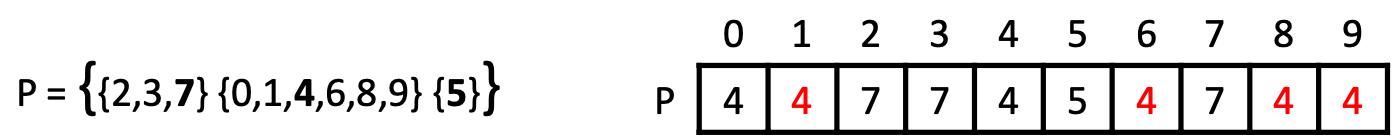
\includegraphics[width=\textwidth]{assets/impPAR2.png}
  \end{center}
  \caption{Resultado implementación vector de pertenencia}
\end{figure}

Vemos que todos los `1' del vector han pasado a ser `4', es decir, todos los elementos que estaban en el subconjunto donde el representante era el valor `1' se han incluido en el subconjunto cuyo representante es el valor `4'.

\textbf{Implementación mediante lista de elementos}

Es una implementación cuya eficiencia espacial es menor (se gasta más espacio).

\begin{figure}[h]
  \begin{center}
    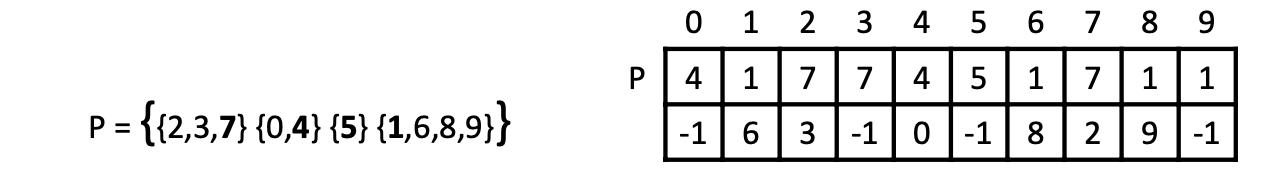
\includegraphics[width=\textwidth]{assets/impPAR3.png}
  \end{center}
  \caption{Ejemplo implementación lista de elementos}
\end{figure}

Ahora almacenamos tanto el `vector de pertenencia' (\(P\)) que contiene el representante de cada subconjunto y un campo que indica que elemento le precede, en el caso del elemento `0' el valor es -1, es decir, no hay más valores en el subconjunto, pero si nos vamos al elemento `8' vemos que su valor es 9, es decir que el elemento `8' precede al elemento `9'.

Queremos realizar la operación \texttt{unir(4,1)}, como vemos en la \textit{Figura 10.4}, tanto el elemento `4' como el `1' son representantes de sus subconjuntos, por tanto si realizamos la unión los valores que suceden a los elementos va a cambiar, quedando:
\begin{figure}[h]
  \begin{center}
    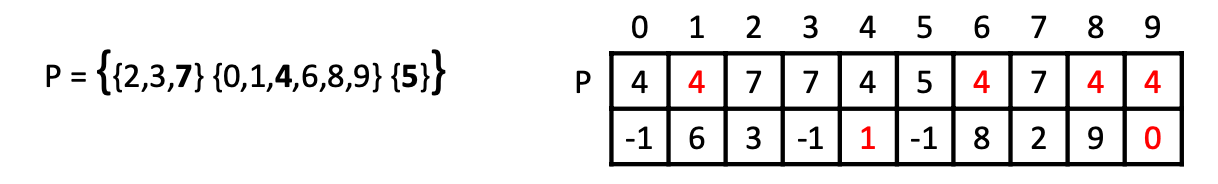
\includegraphics[width=\textwidth]{assets/impPAR4.png}
  \end{center}
  \caption{Resultado implementación lista de elementos}
\end{figure}

Es decir, si nos fijamos en el valor que tenía anteriormente el elemento `4' que era 0, ahora vemos que ese valor es 1 (ahora del elemento 4 vamos al elemento 1), además podemos ver que el representante de los elementos `1', `6', `8' y `9' ahora es `4', el representante del nuevo subconjunto.

El coste de las operaciones son:
\begin{itemize}
  \item \texttt{encontrar()} \(\in O(1)\), porque accedemos a la posición directamente.
  \item \texttt{unir()} \(\in O(n)\), pero el tiempo de ejecución es menor.
\end{itemize}
\newpage
\textbf{Implementación mediante lista de elementos con longitud}

Esta implementación es muy parecida a la anteror, pero contiene un campo más para poder evitar el peor caso.

En este nuevo campo almacenamos la longitud para así evitar unir una lista larga con una corta, haciendo que siempre se una una corta a una larga.

\begin{figure}[h]
  \begin{center}
    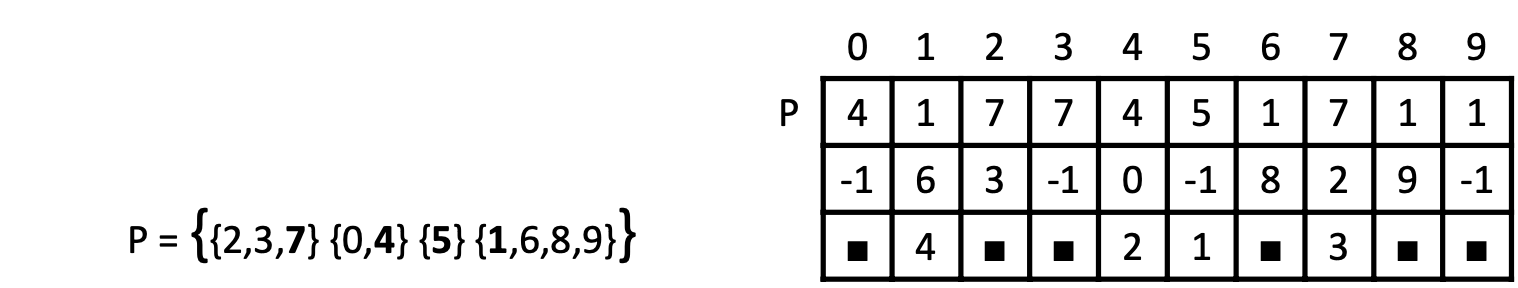
\includegraphics[width=\textwidth]{assets/impPAR5.png}
  \end{center}
  \caption{Ejemplo implementación lista de elementos con longitud}
\end{figure}

Si nos fijamos en la \textit{Figura 10.6} veremos que el elemento `0' su representante es el elemento `4', además es el último elemento del subconjunto, ya que tiene el valor -1 y al ser el último elemento su longitud es `nada' (el cuadro negro), a diferencia del elemento `7' cuyo representante es el elemento `7', su sucesor es el elemento `2' y la longitud es 3 (porque es el número de elementos del subconjunto), solamente los representantes tienen este valor asignado.

Vamos a realizar la operación \texttt{unir(4,1)}:

\begin{figure}[h]
  \begin{center}
    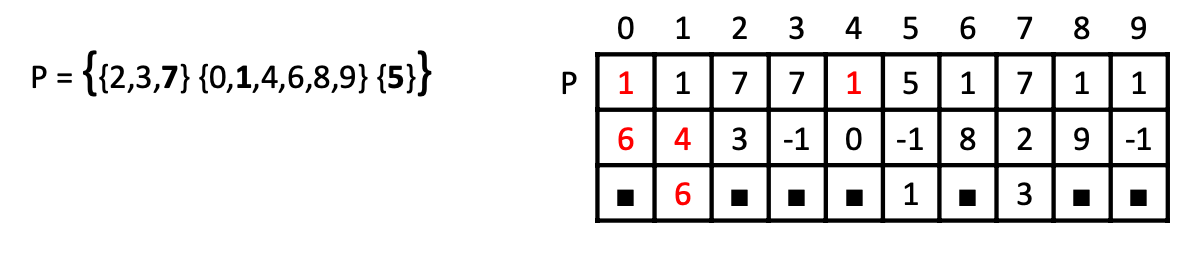
\includegraphics[width=\textwidth]{assets/impPAR6.png}
  \end{center}
  \caption{Resultado implementación lista de elementos con longitud}
\end{figure}

Como vemos, se realizan los mismos cambios que en el ejemplo anterior (\textit{Figura 10.5: Resultado implementación lista de elementos}), pero con el extra de que tenemos que cambiar la longitudes de los representantes.
Al unir los subconjuntos de los elementos `4' y `1' y al ser el nuevo representante del nuevo subconjunto el elemento `1' este cambiará su longitud de 4 a 6.

Porqué es el elemento `1' el nuevo representante y no `4', esto se debe a que ahora unimos el \textbf{subconjunto corto} al \textbf{subconjunto largo}, como el subconjunto cuyo representante era `4' era el corto en comparación al subconjunto con representante `1' obtenemos el resultado del la \textit{Figura 10.7}.

Ahora el coste de las operaciones son:
\begin{itemize}
  \item \texttt{encontrar()} \(\in O(1)\), porque accedemos a la posición directamente.
  \item \texttt{unir()} \(\in O(n)\), pero el tiempo de ejecución se reduce a la mitad.
\end{itemize}
\newpage
\textbf{Implementación mediante bosque de árboles}

Ahora cada subconjunto pasan a ser árboles (lo más ancho posible). En cada posición del vector vamos a encontrar el \textbf{padre} de dicho elemento en el árbol, donde el \textbf{representante} del subconjunto será el nodo \textbf{raíz} de dicho árbol.

Al igual que en los ejemplos anteriores el valor -1 indicará la ausencia de elemento en dicho árbol, en este caso, indicará que ese nodo no tendrá padre y por ende será el representante (nodo ráiz).

\begin{figure}[h]
  \begin{center}
    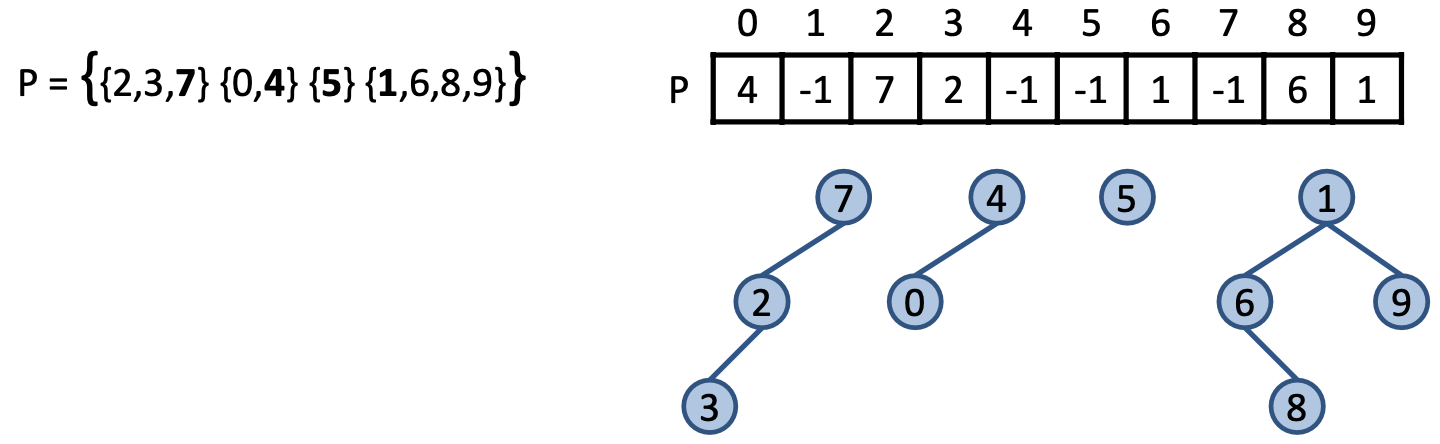
\includegraphics[width=\textwidth]{assets/impPAR7.png}
  \end{center}
  \caption{Ejempo implementación bosque de árboles}
\end{figure}

Ahora si queremos unir los subconjuntos cuyos representantes son 4,1, es decir realizar la operación \texttt{unir(4,1)}, tendríamos que unir el árbol con representante `1' en el árbol con representante `4' o viceversa:
\begin{figure}[h]
  \begin{center}
    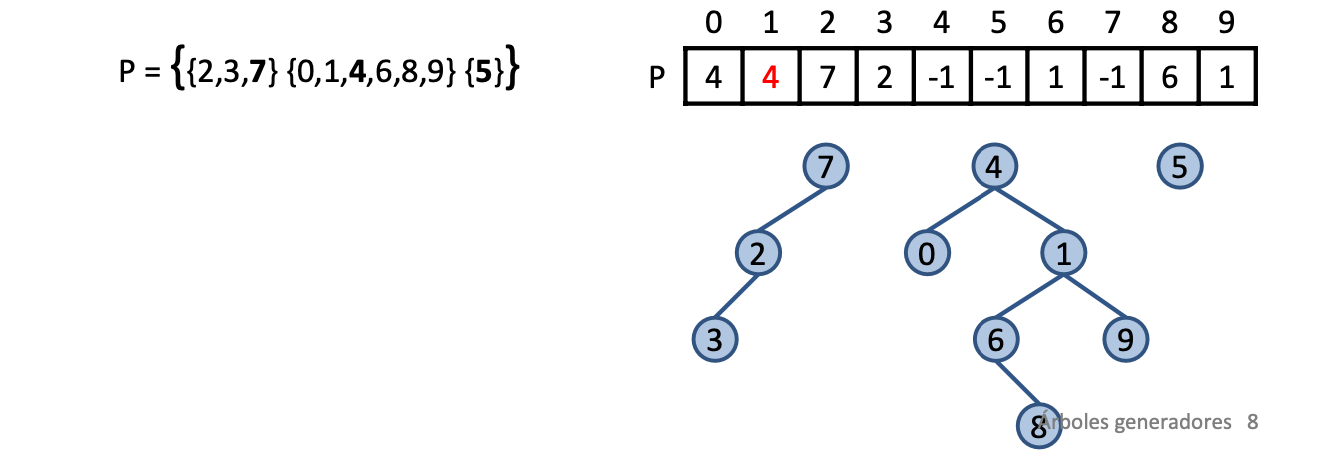
\includegraphics[width=\textwidth]{assets/impPAR9.png}
  \end{center}
  \caption{Resultado implementación bosque de árboles}
\end{figure}

En este caso, hemos unido el árbol del subconjunto con representante `1' al del representante `4' (\textit{Figura 10.9}), es decir el segundo se une al primero.

En este caso el coste de las operaciones son:
\begin{itemize}
  \item \texttt{encontrar()} \(\in O(n)\).
  \item \texttt{unir()} \(\in O(1)\).
\end{itemize}
\newpage
\textbf{Implementación mediante bosque de árboles con control de altura}

Sin embargo, si tenemos árboles (subconjuntos) muy grandes y muy pequeños puede ser muy ineficiente la operación \texttt{unir()}, para poder subsanar este problema encontramos la implementación mediante \textit{bosque de árboles con control de altura}, donde el unimos el árbol más bajo al más alto, ya que la altura no sube (cota).

Una altura inferior \(\rightarrow\) mayor equilibrio del árbol.

Si los árboles tiene la misma altura, da igual quien se una a quien.

Vamos a diferenciar dos tipos de uniónes:
\begin{itemize}
  \item \underbar{\textbf{Unión por tamaño:}}
  El árbol con menos nodos se convierte en el subárbol del que tiene mayor número de nodos.

  Es una alternativa a hacerlo por azar.

  En este caso, lo relevante no es la altura, si no el tamaño de árbol (como su nombre dice), además un error muy común es pensar que mayor tamaño \(\implies\) mayor altura, esto no es así debido a que un árbol general puede tener muchos nodos hermanos y su altura puede seguir siendo 1.

  \item \underbar{\textbf{Unión por altura:}}
  El árbol menos alto se convierte en subárbol del otro.

  Esta implementación es la más acertada, debido a que vamos a unir el árbol `más pequeño' al más `grande', haciendo que el árbol resultante crezca en anchura.
  \begin{figure}[h]
    \begin{center}
      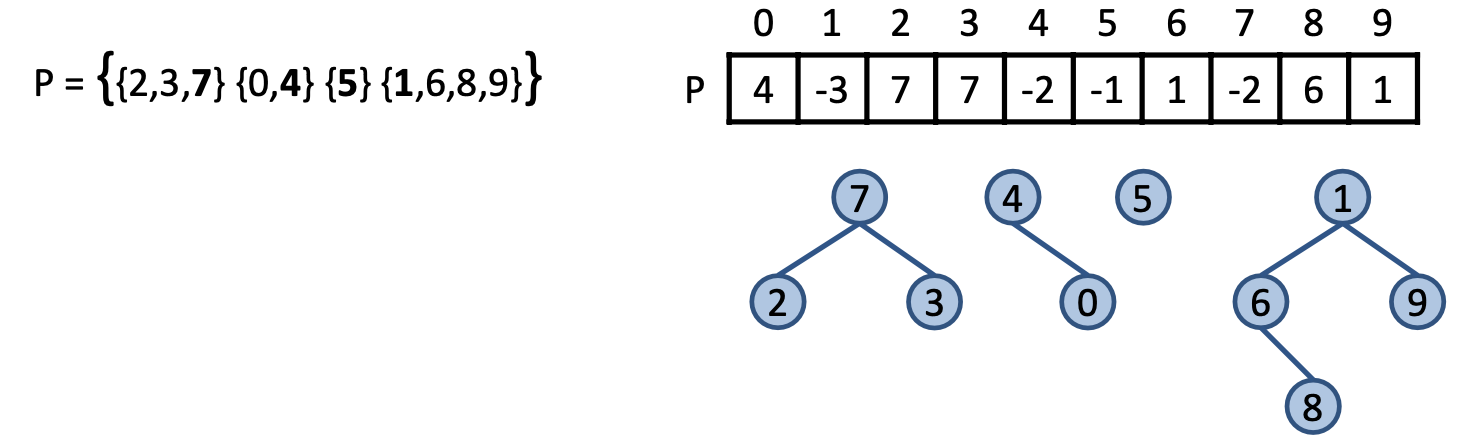
\includegraphics[width=\textwidth]{assets/impPAR11.png}
    \end{center}
    \caption{Ejemplo bosque de árboles control de altura (unión por altura)}
  \end{figure}

Ahora en el vector de pertenencia \(P\), si el nodo padre, encontramos que el valor indica la altura del árbol - 1 (en negativo), es decir, se pone \(-(altura\_arbol-1)\). Cuando la altura es 0 ponemos el valor -1, debido a que encontramos una ambigüedad en el caso de -0.

Ahora al unir dos árboles, la operación \texttt{encontrar()} pasa a ser de coste \(O(log\ n)\), ya que vamos descartando las ramas donde no se encuentra dicho valor.

Vamos a realizar la operación \texttt{unir(4,1)}:

Como vemos en la \textit{Figura 10.10} el árbol con representante (raíz)`4' es mucho más pequeño que el árbol con raíz `1', por tanto, el primero se convertirá en subárbol del árbol con raíz `1', haciendo que el árbol gane anchura y la altura no se vea incrementada (\textit{Figura 10.11}).

Finalmente, vemos que en el vector el contenido del elemento `4' pasa a ser -2(altura del árbol anterior) a 1 (su nodo padre).
\begin{figure}[h]
  \begin{center}
    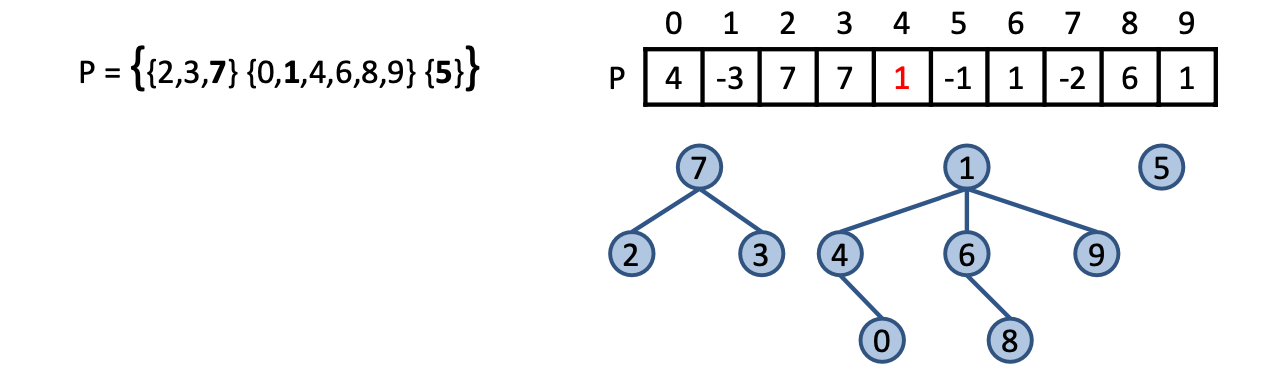
\includegraphics[width=\textwidth]{assets/impPAR12.png}
  \end{center}
  \caption{Resultado bosque de árboles control de altura (unión por altura)}
\end{figure}
Si ambos árboles tienen la misma altura, da igual en el orden que insertemos los subárboles.

\item \underbar{\textbf{Compresión de caminos:}} Optimiza la altura de los árboles.

Ahora con la primera pasada sabemos el representante del nodo `x' a encontrar, en la segunda pasada ya sabemos todos los nodos que pertenecen a dicho representante.

Queremos realizar la operación \texttt{encontrar(20)}:

\begin{figure}[h]
  \begin{center}
    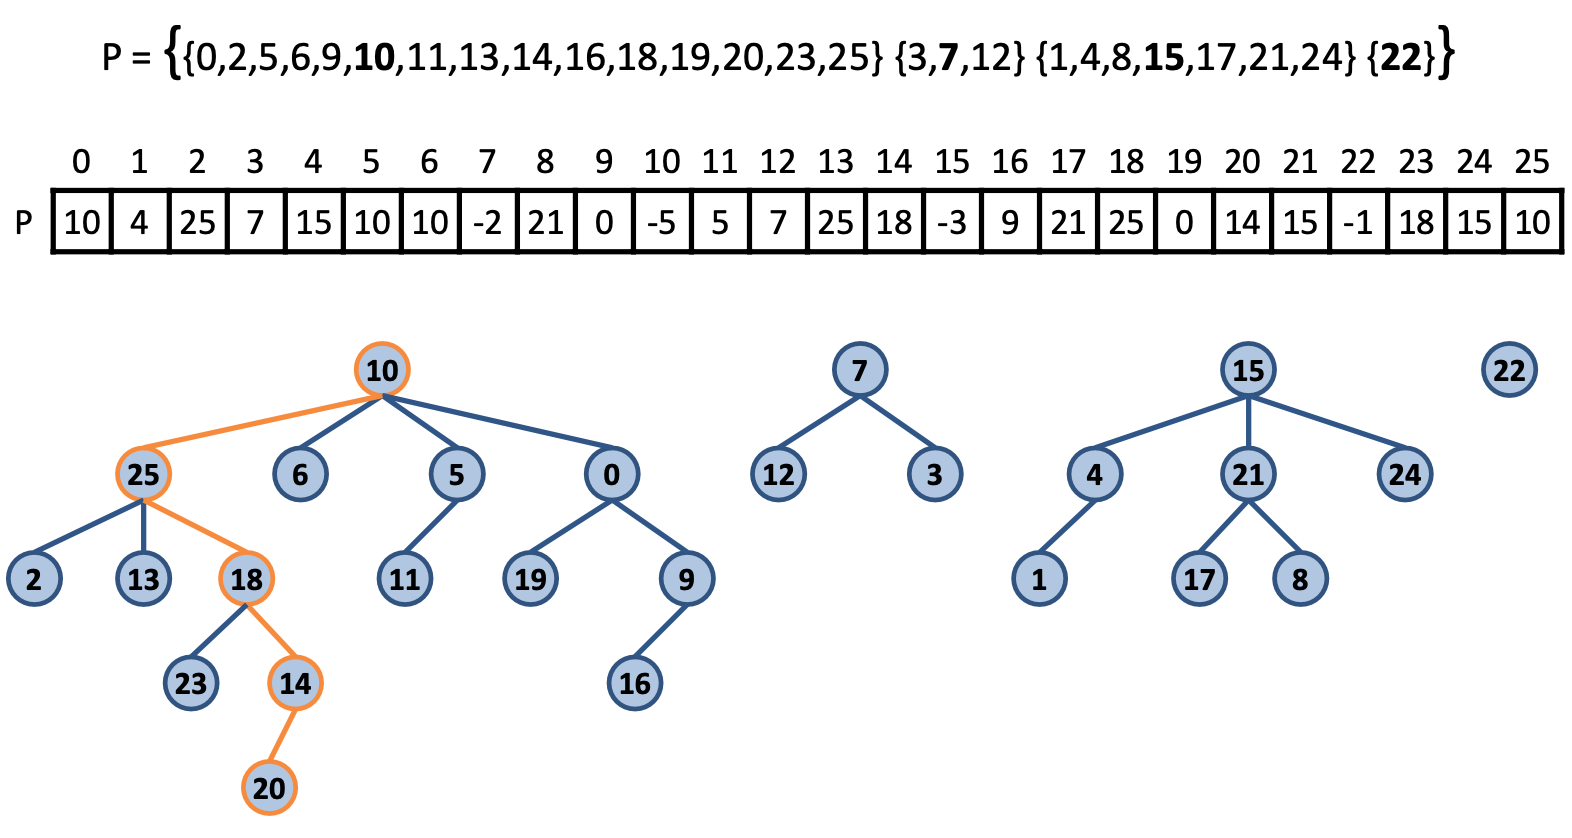
\includegraphics[width=.9\textwidth]{assets/impPAR13.png}
  \end{center}
  \caption{Ejemplo bosque de árboles control de altura (compresión de caminos)}
\end{figure}

En la primera pasada encontramos que el representante del subconjunto de 20, es el elemento `10', en la segunda pasada colocamos el elemento `20' como hijo izquierdo del representante (elemento `10') y así sucesivamente con todos los elementos del subconjunto.

Si nos fijamos en el vector de pertenencia \(P\), el elemento `18' tiene como representante al elemento `10', pero esto no se corresponde con el árbol visto en la \textit{Figura 10.12}, por tanto, vamos a optimizar su altura, haciendo que el nodo con valor `18' sea ahora un hijo del nodo con valor `10', lo mismo con el elemento `14'.

\begin{figure}[h]
  \begin{center}
    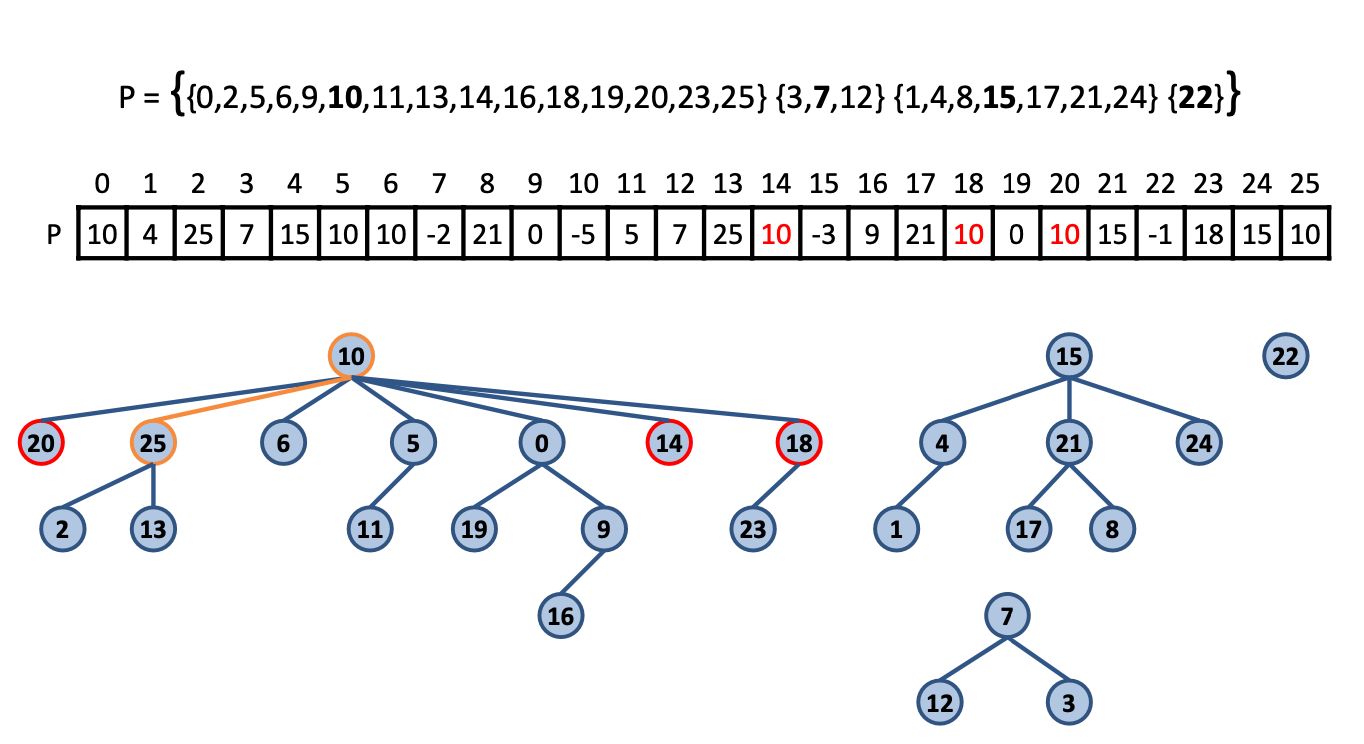
\includegraphics[width=.9\textwidth]{assets/impPAR14.png}
  \end{center}
  \caption{Resultado bosque de árboles control de altura (compresión de caminos)}
\end{figure}

Vemos que los nodos 20,14 y 18 (señalados en rojo) han cambiado de posición en el árbol, disminuyendo la altura e incrementando la anchura del mismo, además si nos fijamos en le vector de pertenencia los valores de elementos 20(14) ,14(18) y 18(25) han cambiado a 10.

Si hiceramos la operación \texttt{encontrar(16)}, tanto el nodo 16, como 9 cambiarían de posición siendo hijos de nodo 10 (su representante).
\end{itemize}

Gracias a esto el coste de las operaciones son:
\begin{itemize}
  \item \texttt{encontrar()} \(O(log\ n)\).
  \item \texttt{unir()} \(\in O(1)\).
\end{itemize}

\textbf{Código de la implementación mediante bosque de árboles control de altura}

\begin{minted}[breaklines]{C++}
class Particion{
  public:
    Particion(int n): padre(n-1){}
    void unir(int a, int b);
    int encontrar(int x)const;
  private:
    mutable std::vector<int>padre;
};

void Particion::unir(int a, int b){
  if(padre[b] < padre[a]){
    padre[a] = b;
  }
  else if(padre[a] == padre[b]){//como aumenta la altura, le restamos 1
    padre[a]--; //árbol resultante tiene un nivel más
    padre[b] = a;
  }
}
int Particion::encontrar(int x)const{
  int y,raiz = x;
  while(padre[raiz] > -1){ //tiene padre y no es representante
    raiz = padre[raiz];
//Compresión del camino: lo nodos del camino se hacen hijos de la raiz.
    while(padre[x]> -1){
      y = padre[x];
      padre[x] =raiz;
      x = y;
    }
  }
  return raiz;
}
\end{minted}




\section{Algoritmo de Kruskal}
Con el \textit{algoritmo de Kruskal} obtenemos un árbol generador de coste mínimo mediante la ordenación de todas las aristas del grafo por su peso (de menor a mayor) y luego añadiendo las que son más baratas (la menores) al árbol de expansión, asegurándose de que no se producen cíclos.

\subsection{Ejemplo algoritmo Kruskal}
Partimos de un grafo ponderado, no dirigido y conexo y guardamos las aristas según su peso.
\begin{figure}[h]
  \begin{center}
    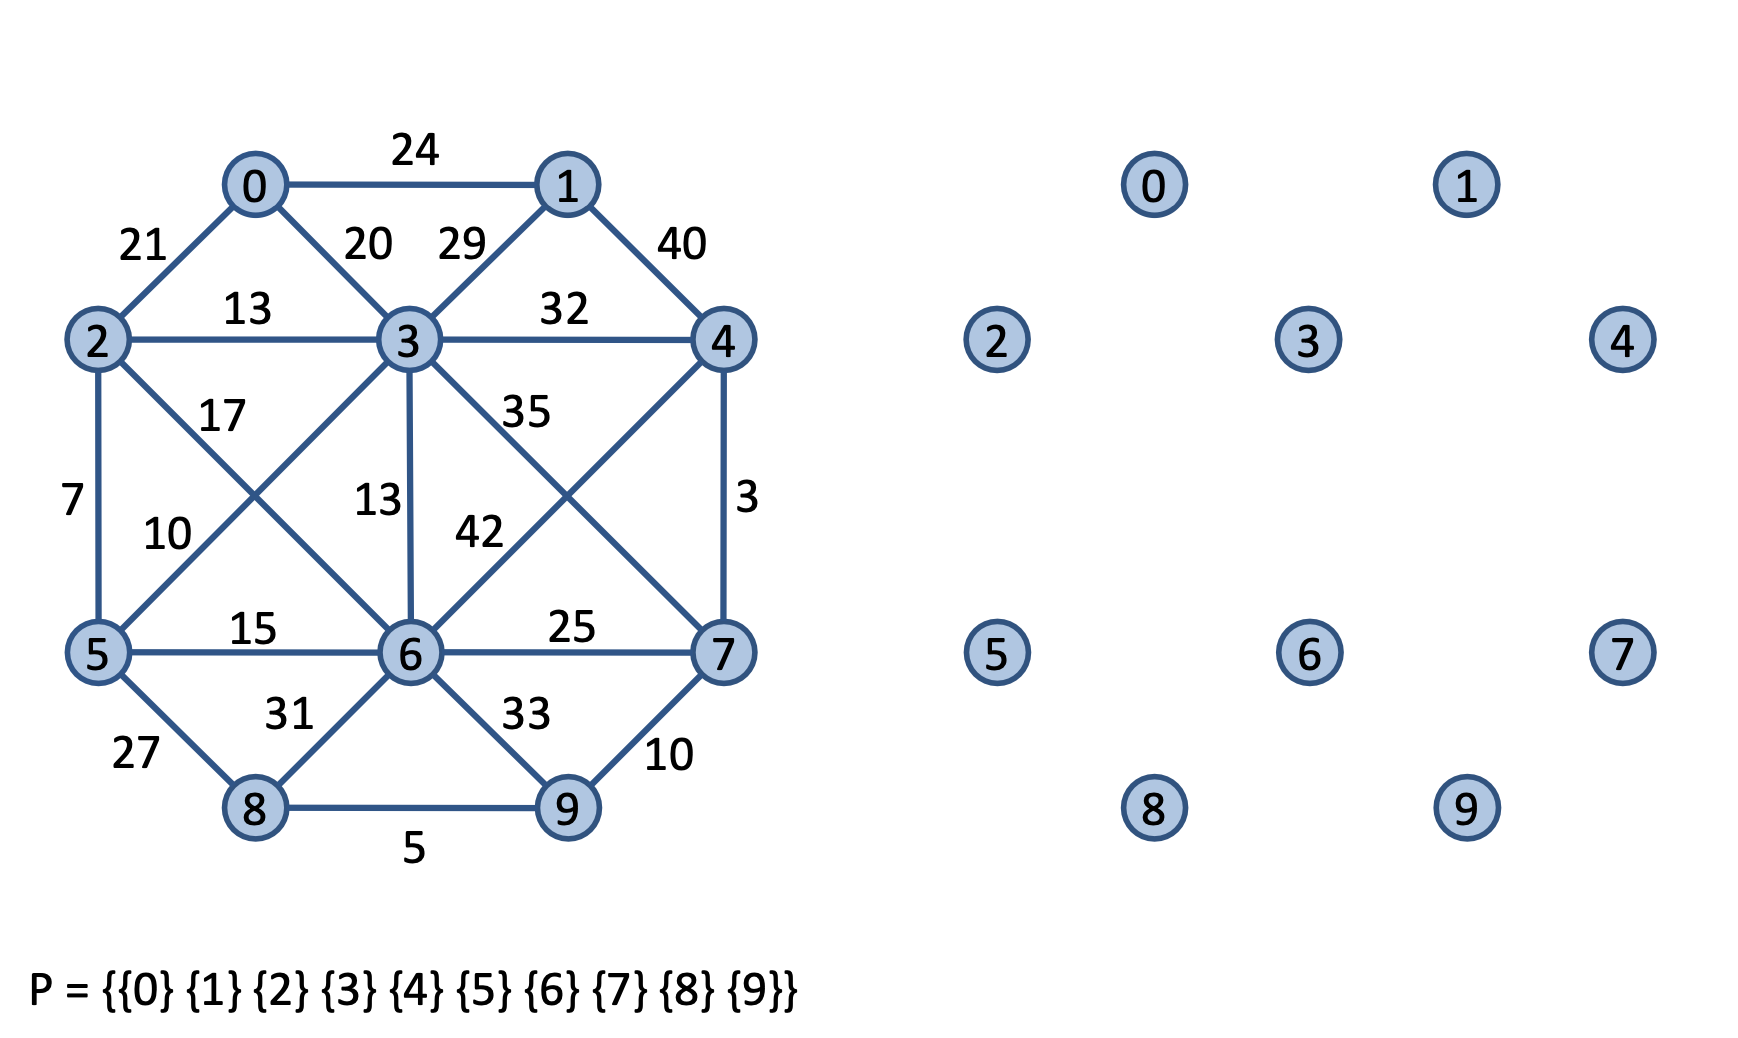
\includegraphics[width=.7\textwidth]{assets/kru1.png}
  \end{center}
  \caption{Ejemplo algoritmo Kruskal}
\end{figure}

Vemos que tenemos el grafo comentado anteriormente, los vértices del mismo pero sin aristas y una partición \(P\) que contiene los subconjuntos a los que pertenece cada elemento (nodo).

Por tanto, para crear obtener el \textit{árbol generador de coste mínimo} cogemos la arista con menor peso y unimos el par de vértices que la contiene, añadiendo en la partición \(P\) los nodos que están unidos en un subconjunto común.

Para ello, vamos a seguir una serie de pasos los cuales como resultado obtendremos el árbol de expansión de coste mínimo:
\begin{enumerate}
  \item Cogemos la arísta con menor coste \(\rightarrow\) \textit{Figura 10.15: Ejemplo 1 Kruskal}.
  \item Unimos los vértices que une dicha arista \(\rightarrow\) realizamos la opración \texttt{unir(P.encontrar(4),\\P.encontrar(7));}, donde buscamos los representantes de cada subconjunto y los unimos (\textit{Figura 10.15.(a)}).
  Si ambos tienen el mismo representante no se unen.
  \item Vemos que los vértices se unen al mismo subconjunto y tienen el mismo representante el cual puede ser el mayor o el menor que unen (\textit{Figura 10.15.(b)}).
  \item Ahora hacemos lo mismo con la siguente arista cuyo valor sea el menor de los valores mayores o igual a la arista anterior (\textit{Figura 10.16.(a)}). 
\end{enumerate}

Para comenzar vamos cogemos la arista cuyo valor sea el más pequeño, este caso será la que une los vértices `4' y `7', con valor 3:
\begin{figure}[h]
  \begin{minipage}{0.4\textwidth}
    \centering
    \begin{subfigure}{\textwidth}
      \centering
      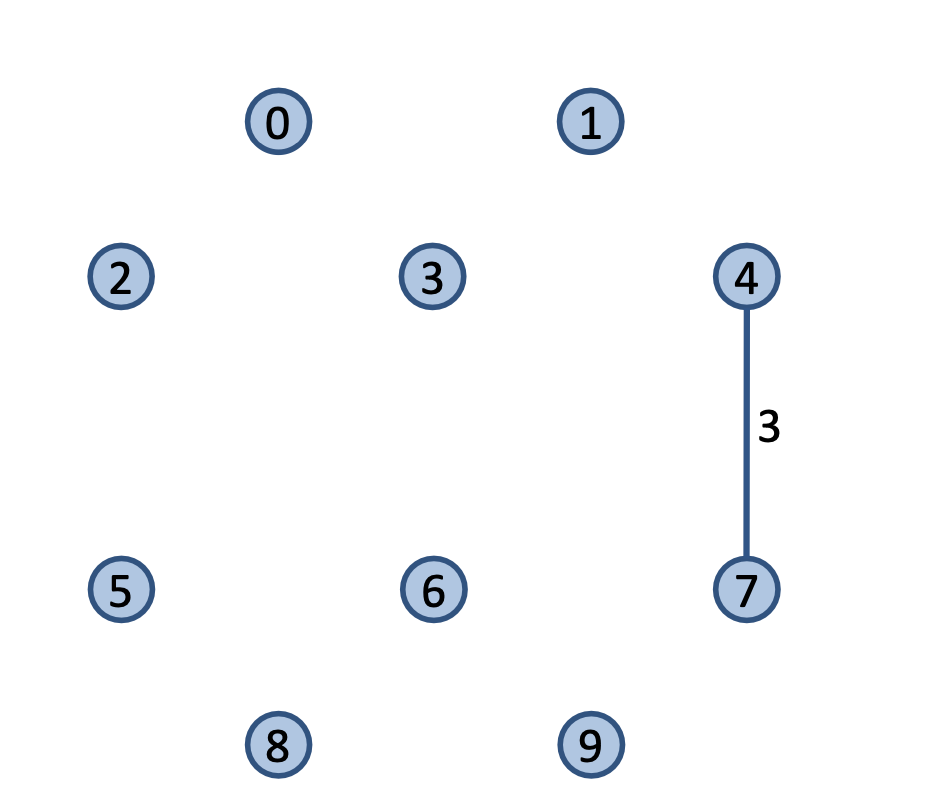
\includegraphics[width=.65\textwidth]{assets/kru2.png}
      \caption{Incluimos la primera arista}
    \end{subfigure}
  \end{minipage}
  \hfill
  \begin{minipage}{0.5\textwidth}
    \centering
    \begin{subfigure}{\textwidth}
      \centering
      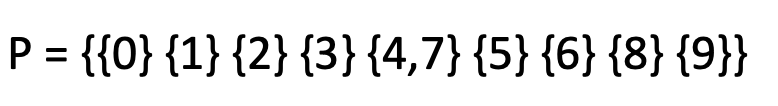
\includegraphics[width=\textwidth]{assets/kru3.png}
      \caption{Incluimos la primera arista que conecta los vértices 4 y 7 y ambos se incluyen en el mismo subconjunto.}
    \end{subfigure}
  \end{minipage}
  \caption{Ejemplo 1 Kruskal}
\end{figure}

Ahora elegimos la siguente arista cuyo valor sea mayor a la de la arista anterior elegida y que no produzca cíclos:
\begin{figure}[h]
  \begin{minipage}{0.4\textwidth}
    \centering
    \begin{subfigure}{\textwidth}
      \centering
      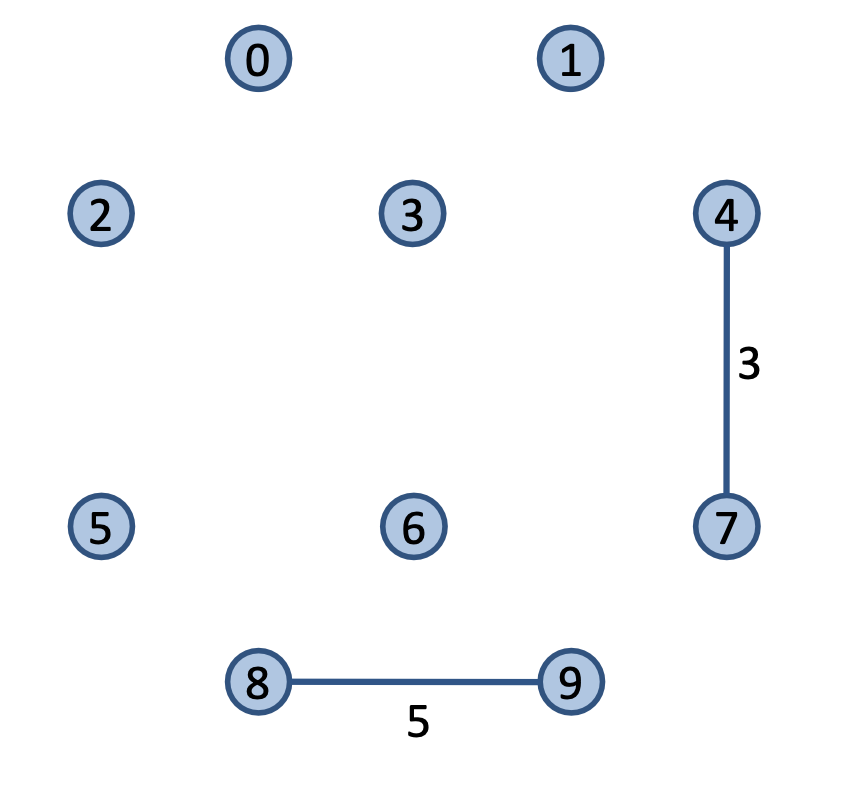
\includegraphics[width=.65\textwidth]{assets/kru5.png}
      \caption{Incluimos la siguente arista con valor \(\geq\) a la anterior}
    \end{subfigure}
  \end{minipage}
  \hfill
  \begin{minipage}{0.5\textwidth}
    \centering
    \begin{subfigure}{\textwidth}
      \centering
      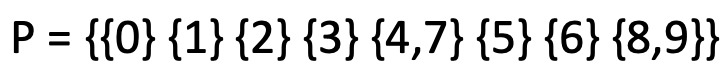
\includegraphics[width=\textwidth]{assets/kru6.png}
      \caption{Se unen los vértices 8 y 9 en el mismo subconjunto}
    \end{subfigure}
  \end{minipage}
  \caption{Ejemplo 2 Kruskal}
\end{figure}

Hacemos esto hasta que tengamos todos los nodos unidos sin ciclos, muy importante debido a que en los árboles no hay ciclos, y como resultado tenemos:

\begin{figure}[h]
  \begin{center}
    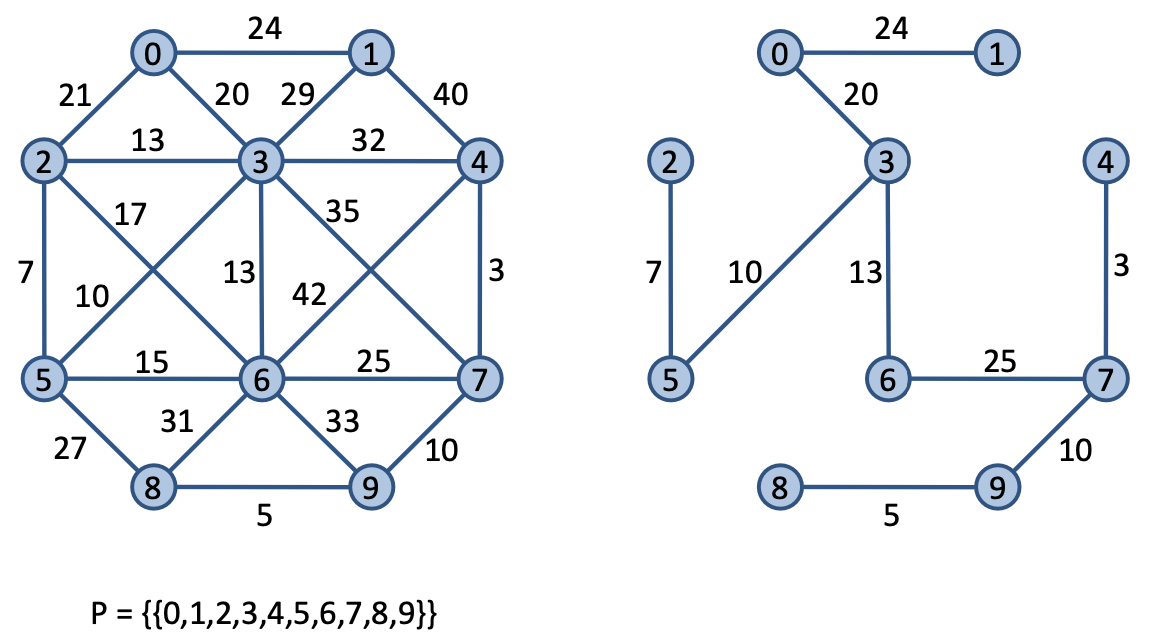
\includegraphics[width=.7\textwidth]{assets/kru4.png}
  \end{center}
  \caption{Resultado ejemplo algoritmo Kruskal}
\end{figure}

Como hemos conseguido una partición que contiene un único subconjunto de vértices, no nos hace falta recorrer más la lista de las aristas ni el grafo debido a que todos los vértices están unidos mediante las aristas con los costes mínimos, en definitiva tenemos termiando el \textit{árbol de expansión de coste mínimo}.



\section{Algoritmo de Prim}
En el \textit{algoritmo de Prim} también vamos a obtener un árbol de expansión de coste mínimo pero usando otra metodología.

Ahora, en vez de tener una partición donde se encuentran todos los vértices del grafo y se va cogiendo la arista con menor valor, vamos a tener un vector de booleanos \(U\) que indicará porqué vértices hemos pasado y se empezará desde el vértice con menor coste.

\begin{figure}[h]
  \begin{center}
    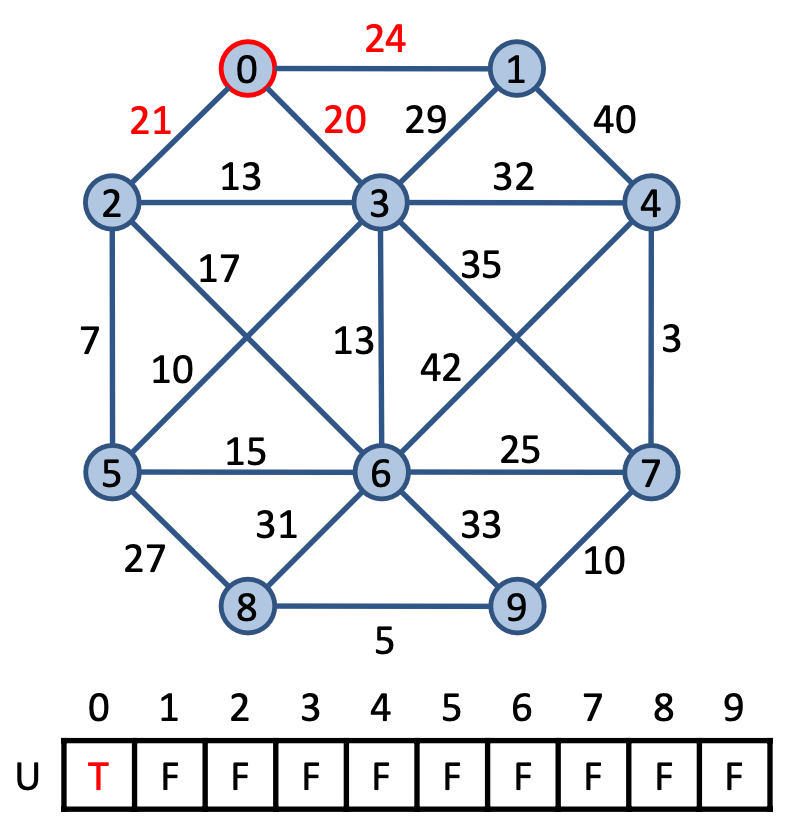
\includegraphics[width=.5\textwidth]{assets/prim1.png}
  \end{center}
  \caption{Ejemplo del algoritmo Prim}
\end{figure}
\newpage
Vemos que partimos desde el vértice con valor 0 y que tenemos 3 aristas disponibles con costes (20, 21 y 24), lo que vamos a hacer es pasar por la arista que tenga menor coste, es decir, por la de coste 20 uniendo los vértices (0 y 3) y las otras dos restantes quedaría `eliminadas'.

\begin{figure}[h]
  \begin{minipage}{0.4\textwidth}
    \centering
    \begin{subfigure}{\textwidth}
      \centering
      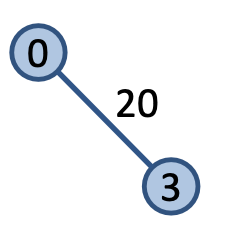
\includegraphics[width=.5\textwidth]{assets/prim2.png}
      \caption{Unimos ambos vértices con la arista de menor coste.}
    \end{subfigure}
  \end{minipage}
  \hfill
  \begin{minipage}{0.5\textwidth}
    \centering
    \begin{subfigure}{\textwidth}
      \centering
      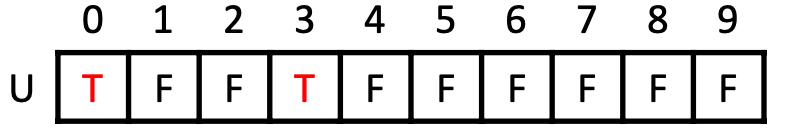
\includegraphics[width=\textwidth]{assets/prim3.png}
      \caption{Ponemos en T (true) los vértices por los que hemos pasado.}
    \end{subfigure}
  \end{minipage}
  \caption{Ejemplo 1 Prim}
\end{figure}

Ahora nos encontramos en el vértice `3' y si nos fijamos en el grafo de la \textit{Figura 10.17} vemos que se puede unir con varios vértices (\(3 \leftrightarrow 2\) con coste 13), (\(3 \leftrightarrow 6\) con coste 13) y (\(3 \leftrightarrow 5\) con coste 10), como la arista de menor coste es 10, uniremos (\(3 \leftrightarrow 5\)).

\begin{figure}[h]
  \begin{minipage}{0.4\textwidth}
    \centering
    \begin{subfigure}{\textwidth}
      \centering
      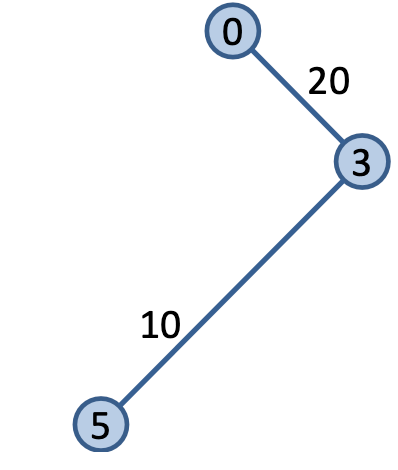
\includegraphics[width=.5\textwidth]{assets/prim5.png}
      \caption{Unimos 3 y 5.}
    \end{subfigure}
  \end{minipage}
  \hfill
  \begin{minipage}{0.5\textwidth}
    \centering
    \begin{subfigure}{\textwidth}
      \centering
      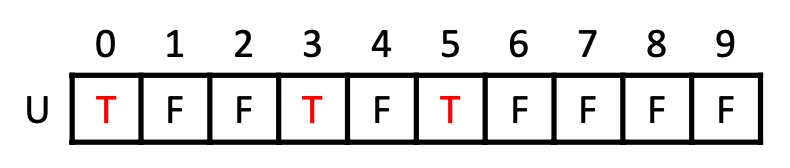
\includegraphics[width=.8\textwidth]{assets/prim6.png}
      \caption{Ponemos en T (true) en el vértice 5.}
    \end{subfigure}
  \end{minipage}
  \caption{Ejemplo 2 Prim}
\end{figure}

Ahora encontramos un problema, tras haber unido los vértices (2 y 5) nos encontramos en el vértices `2', pero no podemos unirlo con nigún vertice ya que si lo unimos con los vértices (0,3) tendríamos un ciclo.
\begin{figure}[h]
  \begin{minipage}{0.4\textwidth}
    \centering
    \begin{subfigure}{\textwidth}
      \centering
      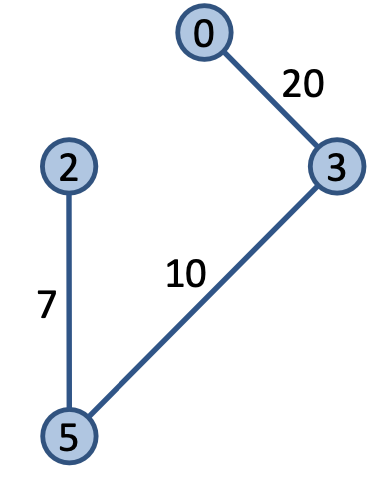
\includegraphics[width=.5\textwidth]{assets/prim9.png}
    \end{subfigure}
  \end{minipage}
  \hfill
  \begin{minipage}{0.5\textwidth}
    \centering
    \begin{subfigure}{\textwidth}
      \centering
      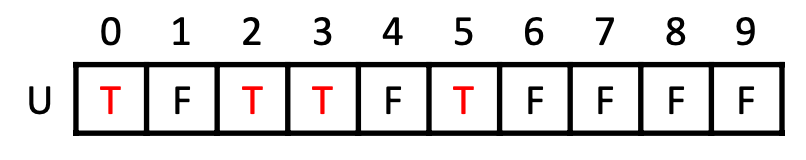
\includegraphics[width=.8\textwidth]{assets/prim10.png}
    \end{subfigure}
  \end{minipage}
  \caption{Ejemplo 3 Prim}
\end{figure}
\newpage
Si nos fijamos en el grafo de ejemplo (\textit{Figura 10.17}) vamos que el vértice 2 se puede unir con el 6 (\(2 \leftrightarrow 6\) con coste 17), pero es que el vértice 3 también se puede unir con 6 (\(3 \leftrightarrow 6\) con coste 13), como el coste de este último es menor, saltamos del vértice 2 al 3 y unimos con el vértice 6.

\begin{figure}[h]
  \begin{minipage}{0.4\textwidth}
    \centering
    \begin{subfigure}{\textwidth}
      \centering
      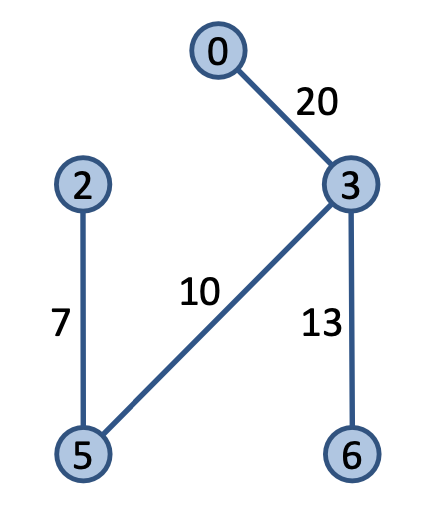
\includegraphics[width=.5\textwidth]{assets/prim11.png}
      \caption{Unimos 3 y 6}
    \end{subfigure}
  \end{minipage}
  \hfill
  \begin{minipage}{0.5\textwidth}
    \centering
    \begin{subfigure}{\textwidth}
      \centering
      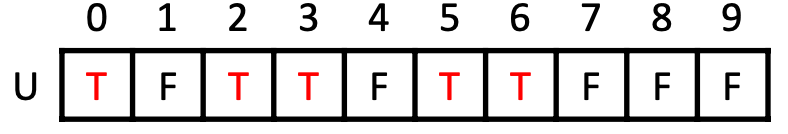
\includegraphics[width=.8\textwidth]{assets/prim12.png}
      \caption{Ponemos en T (true) en el vértice 6.}
    \end{subfigure}
  \end{minipage}
  \caption{Ejemplo 4 Prim}
\end{figure}

Ahora vemos que podemos unir los vertices 6 y 7 (\(6 \leftrightarrow 7\) con coste 25), pero también podemos saltar al vértice 0 y unirlo con 1 (\(0 \leftrightarrow 1\) con coste 24), como la arista de éste último tiene menor coste y por tanto, se unen primero dichos vértices y luego unimos 6 con 7.
\begin{figure}[h]
  \begin{minipage}{0.4\textwidth}
    \centering
    \begin{subfigure}{\textwidth}
      \centering
      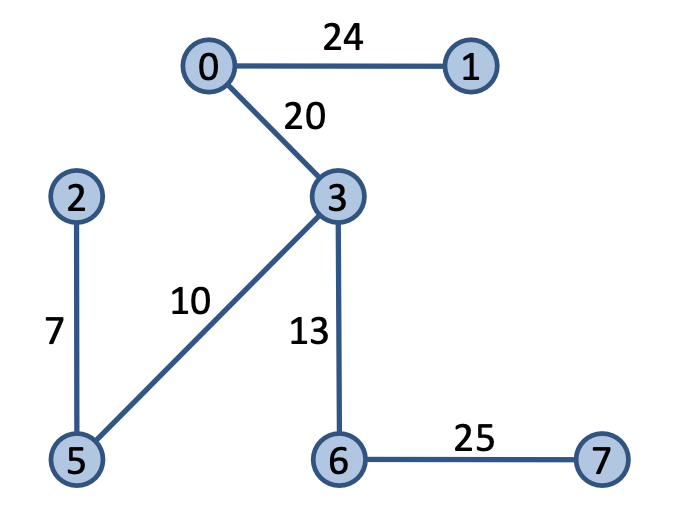
\includegraphics[width=.5\textwidth]{assets/prim13.png}
      \caption{Unimos primero 0 y 1 y luego 6 y 7.}
    \end{subfigure}
  \end{minipage}
  \hfill
  \begin{minipage}{0.5\textwidth}
    \centering
    \begin{subfigure}{\textwidth}
      \centering
      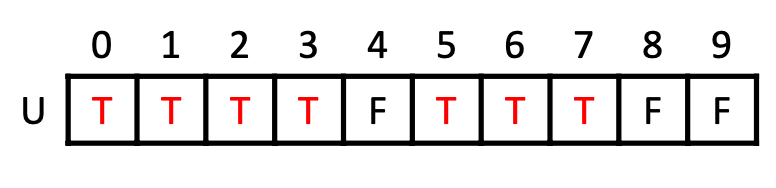
\includegraphics[width=.8\textwidth]{assets/prim14.png}
      \caption{Ponemos en T (true) en el vértice 1 y 7.}
    \end{subfigure}
  \end{minipage}
  \caption{Ejemplo 5 Prim}
\end{figure}

Seguimos uniendo vértices teniendo en cuenta el peso de las aristas y tenemos como resultado final:
\begin{figure}[h]
  \begin{minipage}{0.4\textwidth}
    \centering
    \begin{subfigure}{\textwidth}
      \centering
      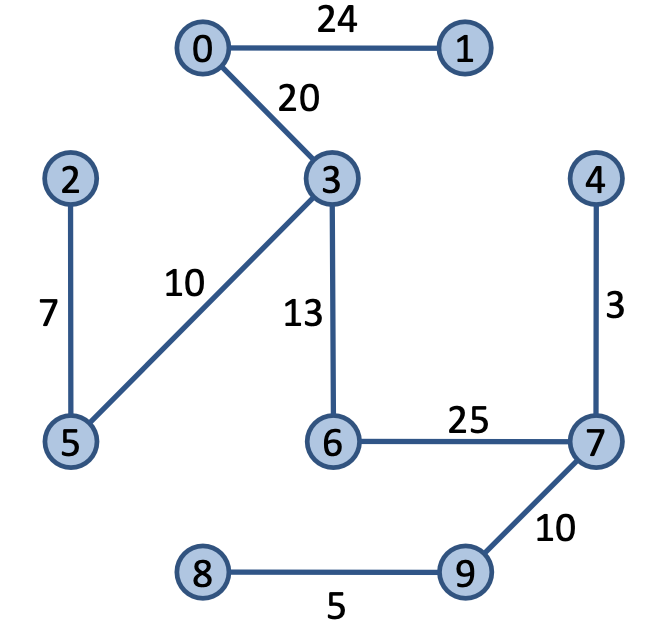
\includegraphics[width=.5\textwidth]{assets/prim15.png}
      \caption{Todos los nodos unidos sin ciclos.}
    \end{subfigure}
  \end{minipage}
  \hfill
  \begin{minipage}{0.5\textwidth}
    \centering
    \begin{subfigure}{\textwidth}
      \centering
      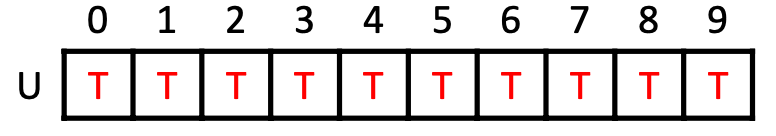
\includegraphics[width=.8\textwidth]{assets/prim16.png}
      \caption{Vector de booleano con todos a T (true).}
    \end{subfigure}
  \end{minipage}
  \caption{Resultado ejemplo de algoritmo Prim}
\end{figure}

Como vemos en las figuras (\textit{Figura 10.17: Resultado ejemplo algoritmo Kruskal}) y (\textit{Figura 11.24: Resultado ejemplo algoritmo Prim}) ambos grafos son idénticos, sin embargo, pueden existir casos en que sean diferentes.

Esto es debido a que aunque Kruskal y Prim trabajen con metodologías diferentes pueden devolver el mismo \textit{árbol de expansión de coste mínimo}, ya que al estar uniendo vértices cuya aristas son las de menor coste es muy probable que el resultado sea el mismo.

Es decir, \textit{Kruskal} y \textit{Prim} hacen lo mismo pero de menera diferente.
